\documentclass[12pt,compress,ngerman,utf8,t]{beamer}
\usepackage[ngerman]{babel}
\usepackage{multicol}
\usepackage{animate}
\usepackage[protrusion=true,expansion=true]{microtype}

\DeclareSymbolFont{extraup}{U}{zavm}{m}{n}
\DeclareMathSymbol{\varheart}{\mathalpha}{extraup}{86}
\DeclareMathSymbol{\vardiamond}{\mathalpha}{extraup}{87}

\title{Jugend hackt}
\author{Ingo Blechschmidt}
\date{Augsburger Linux-Infotag am 28. März 2015}

\usetheme{Warsaw}

\useinnertheme{rectangles}

\usecolortheme{seahorse}
\definecolor{mypurple}{RGB}{150,0,255}
\setbeamercolor{structure}{fg=mypurple}

\usefonttheme{serif}
\usepackage{bookman}

\setbeamertemplate{navigation symbols}{}
\setbeamertemplate{headline}{}
\setbeamertemplate{frametitle}[default][colsep=-2bp,rounded=false,shadow=false,center]

\renewcommand*\insertshorttitle{Augsburger Linux-Infotag am 28. März 2015}

\newcommand{\hil}[1]{{\usebeamercolor[fg]{item}{\textbf{#1}}}}

\begin{document}

\begin{frame}\begin{center}
  \bigskip
  \bigskip
  
\includegraphics[scale=0.6]{images/titel}

  \bigskip
  \small
  Ingo Blechschmidt

  \medskip
  \scriptsize
  Augsburger Linux-Infotag am 28. März 2015
\end{center}\end{frame}

\newcommand{\imgslide}[1]{
  \begin{frame}\frametitle{Jugend hackt}
    \vfill
    \begin{center}
      \includegraphics[width=0.8\textwidth]{images/#1}
    \end{center}
    \vfill

    \transdissolve
    \transduration{10}
  \end{frame}
}

\imgslide{jugend-hackt-0}
\imgslide{jugend-hackt-1}
\imgslide{jugend-hackt-2}
\imgslide{jugend-hackt-3}
\imgslide{jugend-hackt-4}
\imgslide{jugend-hackt-5}
\imgslide{jugend-hackt-6}
\imgslide{jugend-hackt-7}
\imgslide{jugend-hackt-8}
%\imgslide{jugend-hackt-0}
%\imgslide{jugend-hackt-1}
%\imgslide{jugend-hackt-2}
%\imgslide{jugend-hackt-3}
%\imgslide{jugend-hackt-4}
%\imgslide{jugend-hackt-5}
%\imgslide{jugend-hackt-6}
%\imgslide{jugend-hackt-7}
%\imgslide{jugend-hackt-8}
%\imgslide{jugend-hackt-0}
%\imgslide{jugend-hackt-1}
%\imgslide{jugend-hackt-2}
%\imgslide{jugend-hackt-3}
%\imgslide{jugend-hackt-4}
%\imgslide{jugend-hackt-5}
%\imgslide{jugend-hackt-6}
%\imgslide{jugend-hackt-7}
%\imgslide{jugend-hackt-8}

\begin{frame}\frametitle{Mathecamp in den Ferien \\[-0.4em] \scriptsize vom 22. bis 27. August 2015 in Violau}
  \vspace{-0.4cm}
  \begin{center}
    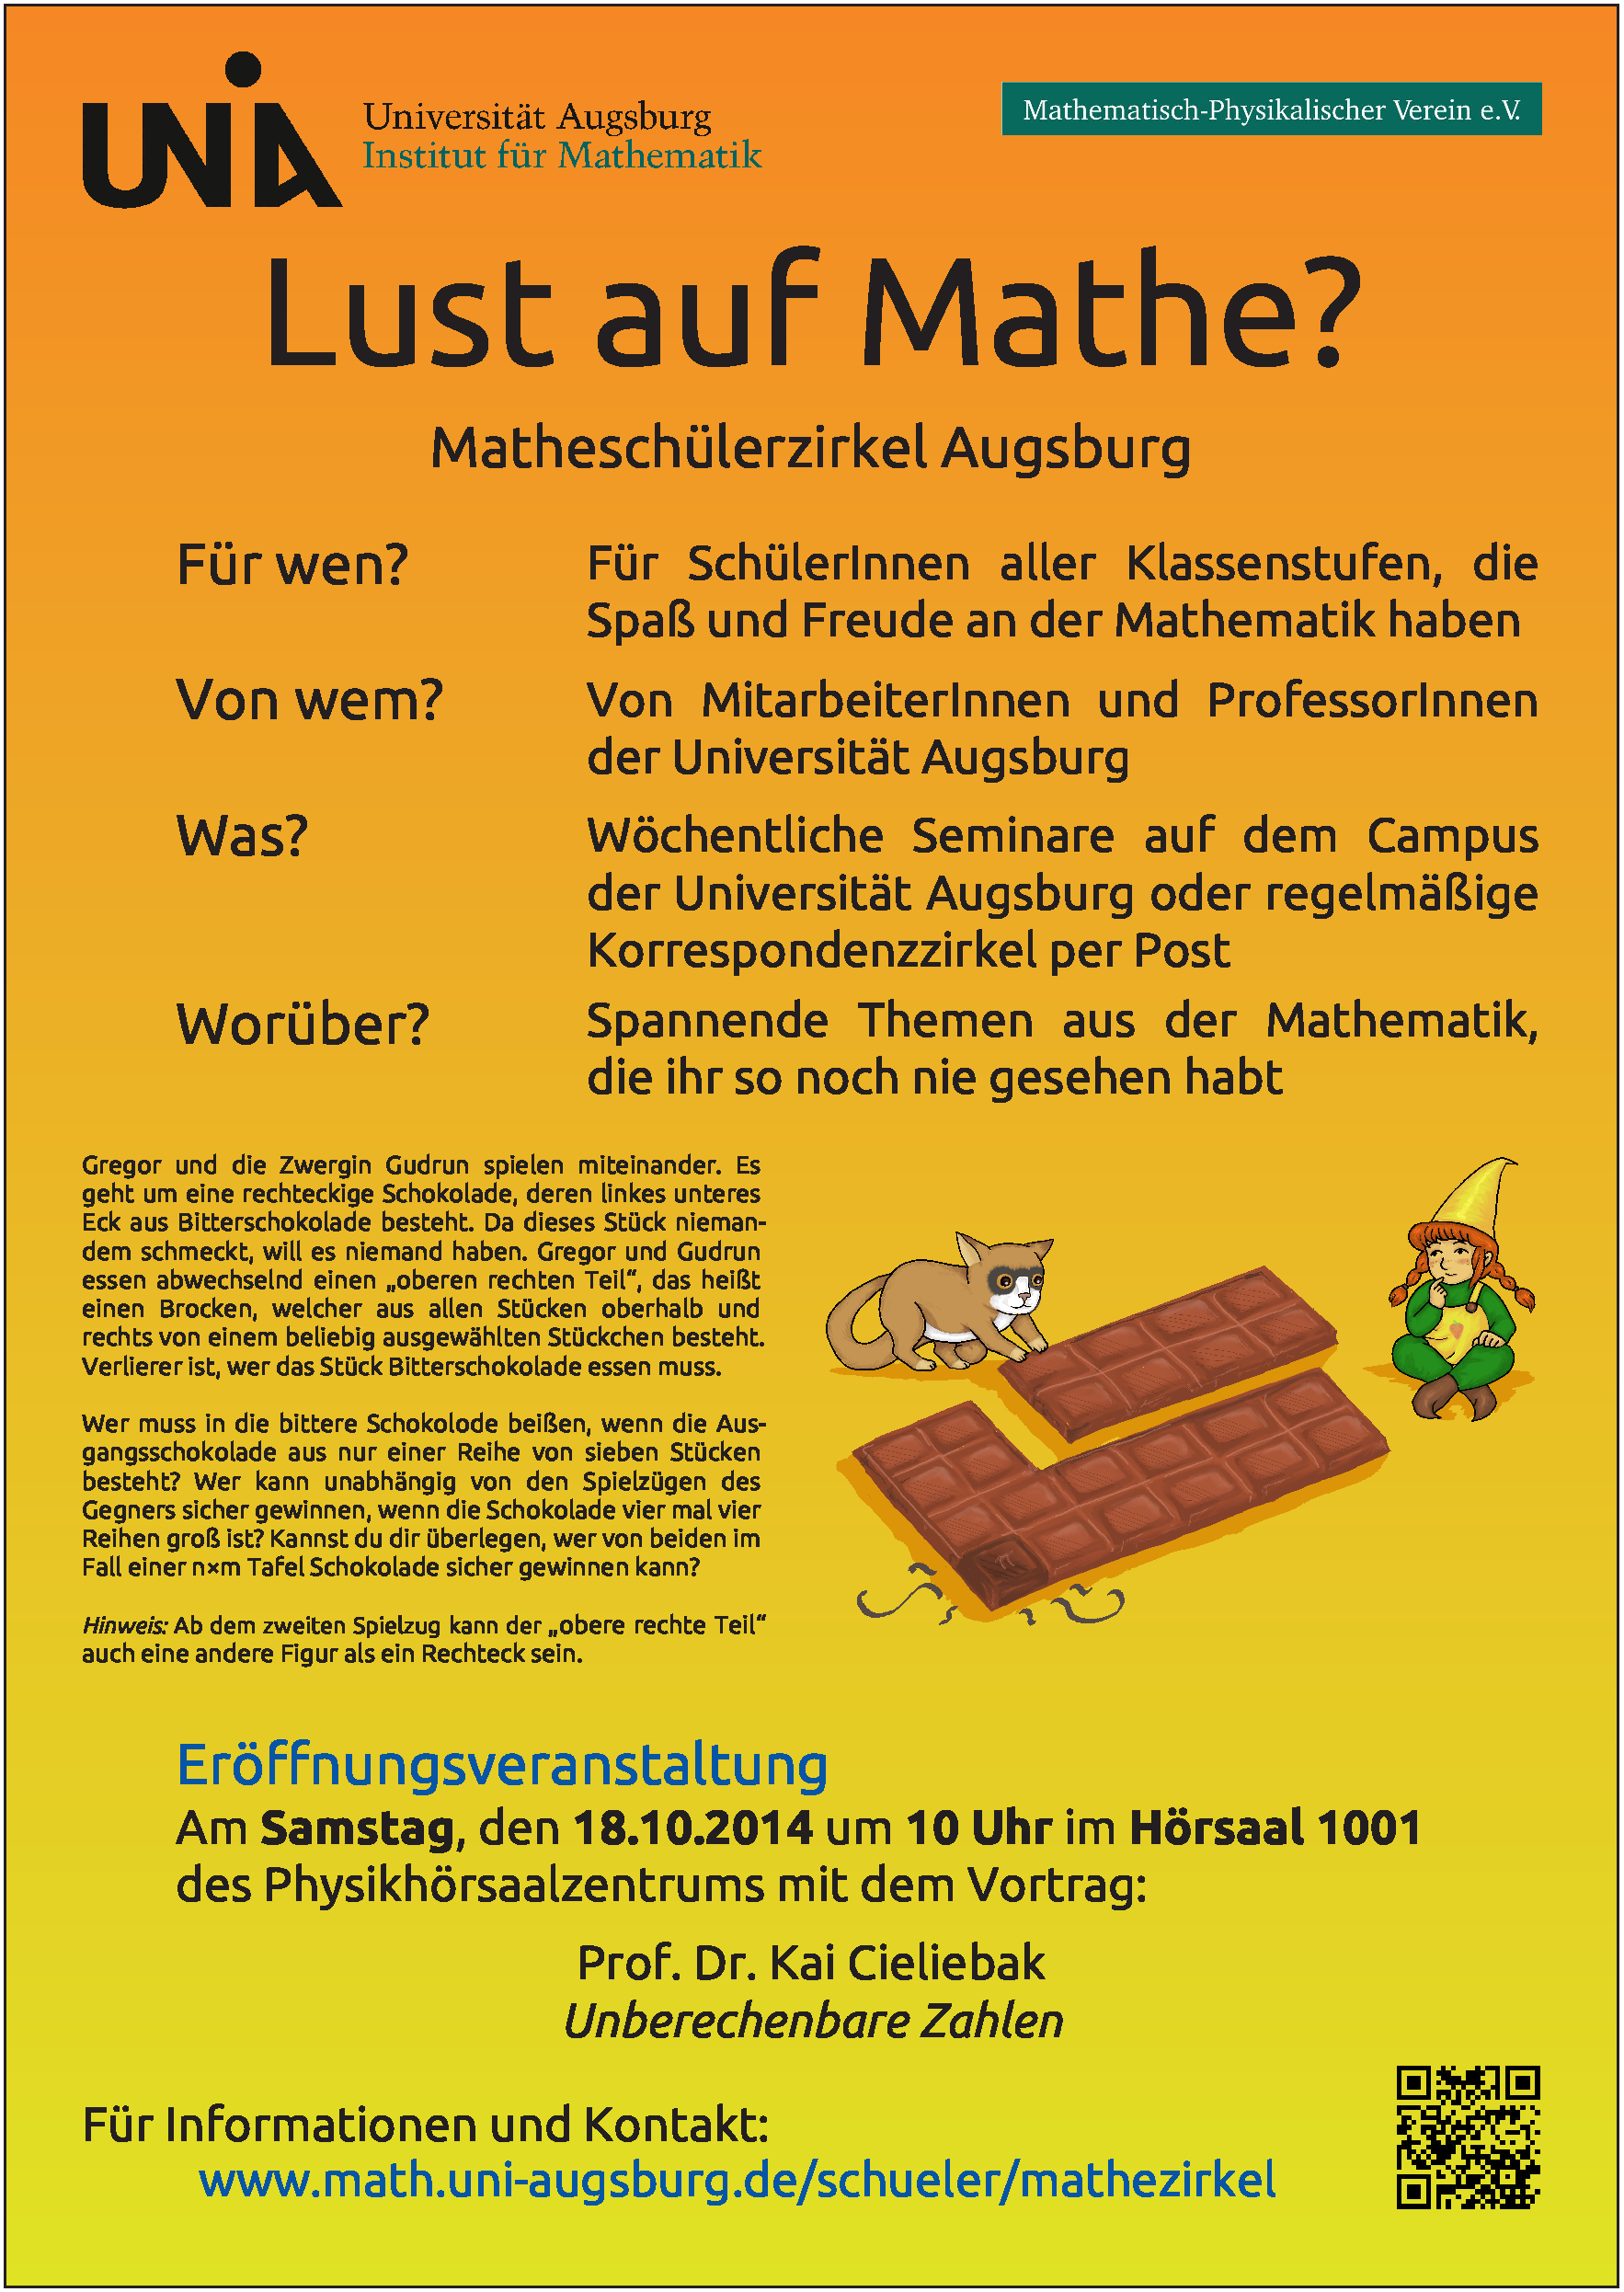
\includegraphics[scale=0.18]{images/mathezirkel}
  \end{center}
\end{frame}

\end{document}
